\section{JPS+}
Jumping from one point to another in the grid avoids many unnecessary A* open
list operations and, as we will show in Section~\ref{cha::jps::results}, can
dramatically improve the performance of online pathfinding search.
Identifying these jump points often requires inspecting large sections of the
grid checking for forced neighbours. Though such operations usually take very
little time the procedure is nevertheless a bottleneck for the algorithm.  In
this section we develop JPS+: a variant of Jump Point Search which
pre-processes the map and replaces each adjacent neighbour of a grid node with
a jump point that lies in the same relative direction. The result of the
pre-processing is an adjacency list data structure that allows computing the
jump point successors of arbitrary nodes in constant time.


\begin{figure}[tb]
       \begin{center}
		   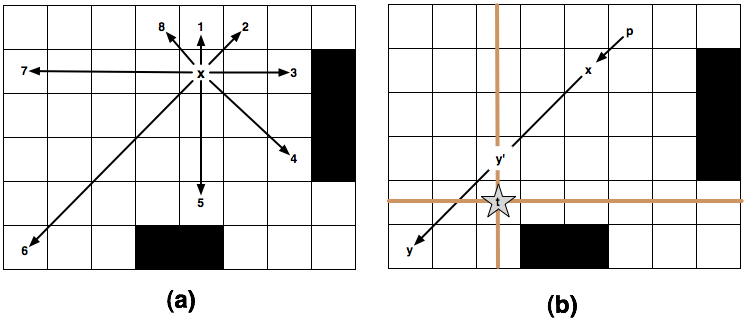
\includegraphics[width=0.95\columnwidth]
			{chapter_jps/diagrams/preproc.png}
       \end{center}
	\vspace{-3pt}
       \caption{(a) A jump point is computed in place of each grid neighbour of node $x$.
		(b) When jumping from $x$ to $y$ we may cross the row or column of the target $t$ (here, both). 
To avoid jumping over $t$ we insert an intermediate successor $y'$ on the row or column of $t$ (whichever is closest to $x$).}

       \label{fig:preproc}
\end{figure}

Figure~\ref{fig:preproc}(a) illustrates our graph reformulation idea for a 
single node $x$. We simply search for a jump point in the direction
of each grid neighbour of $x$. In JPS, we discard all nodes along a failed
path. By comparison, JPS+ must store the last node along a failed path.
These \emph{sterile jump points} are required 
to guarantee optimality during search but are never added to the A* open list.
To see why they are necessary, consider Figure~\ref{fig:preproc}(b).
Here we reach $x$ from $p$ and try to jump from $x$ to $y$. 
Notice that each such jump may cross the goal or column of the target node
$t$. In JPS the diagonal recursion would have terminated at node $y'$, having detected
the goal $t$ along a non-failed straight jump.
JPS+ simulates this behaviour by explicitly inserting an intermediate node $y'$ 
at the point where the jump to $y$ crosses the column of $t$.
This condition is sufficient to preserve optimality during search. The proof
involves showing that JPS+ simulates exactly the behaviour of JPS. We omit it 
for brevity.

\subsection{Properties}
JPS+ requires an offline pre-processing step that has quadratic time complexity
and linear space requirements w.r.t the number of nodes in the grid.

